\usepackage{booktabs}
\hyphenation{thatshouldnot}

\usepackage{makeidx}
\makeindex

\newcommand{\subtitle}[1]{
  \gdef\@subtitle{#1}
}

\renewcommand{\maketitlepage}{%
  \cleardoublepage%
  {%
  \sffamily%
  \begin{fullwidth}%
  \fontsize{18}{20}\selectfont\par\noindent\textcolor{darkgray}{\allcaps{\thanklessauthor}}%
  \vspace{7.5pc}%
  \fontsize{36}{40}\selectfont\par\noindent\textcolor{darkgray}{\allcaps{Introduction to\break Empirical Bayes}}%
  \vspace{5pc}%
  \fontsize{18}{20}\selectfont\par\noindent\textcolor{darkgray}{Examples from Baseball Statistics}%
  \vspace{6pc}%
  \begin{center}
  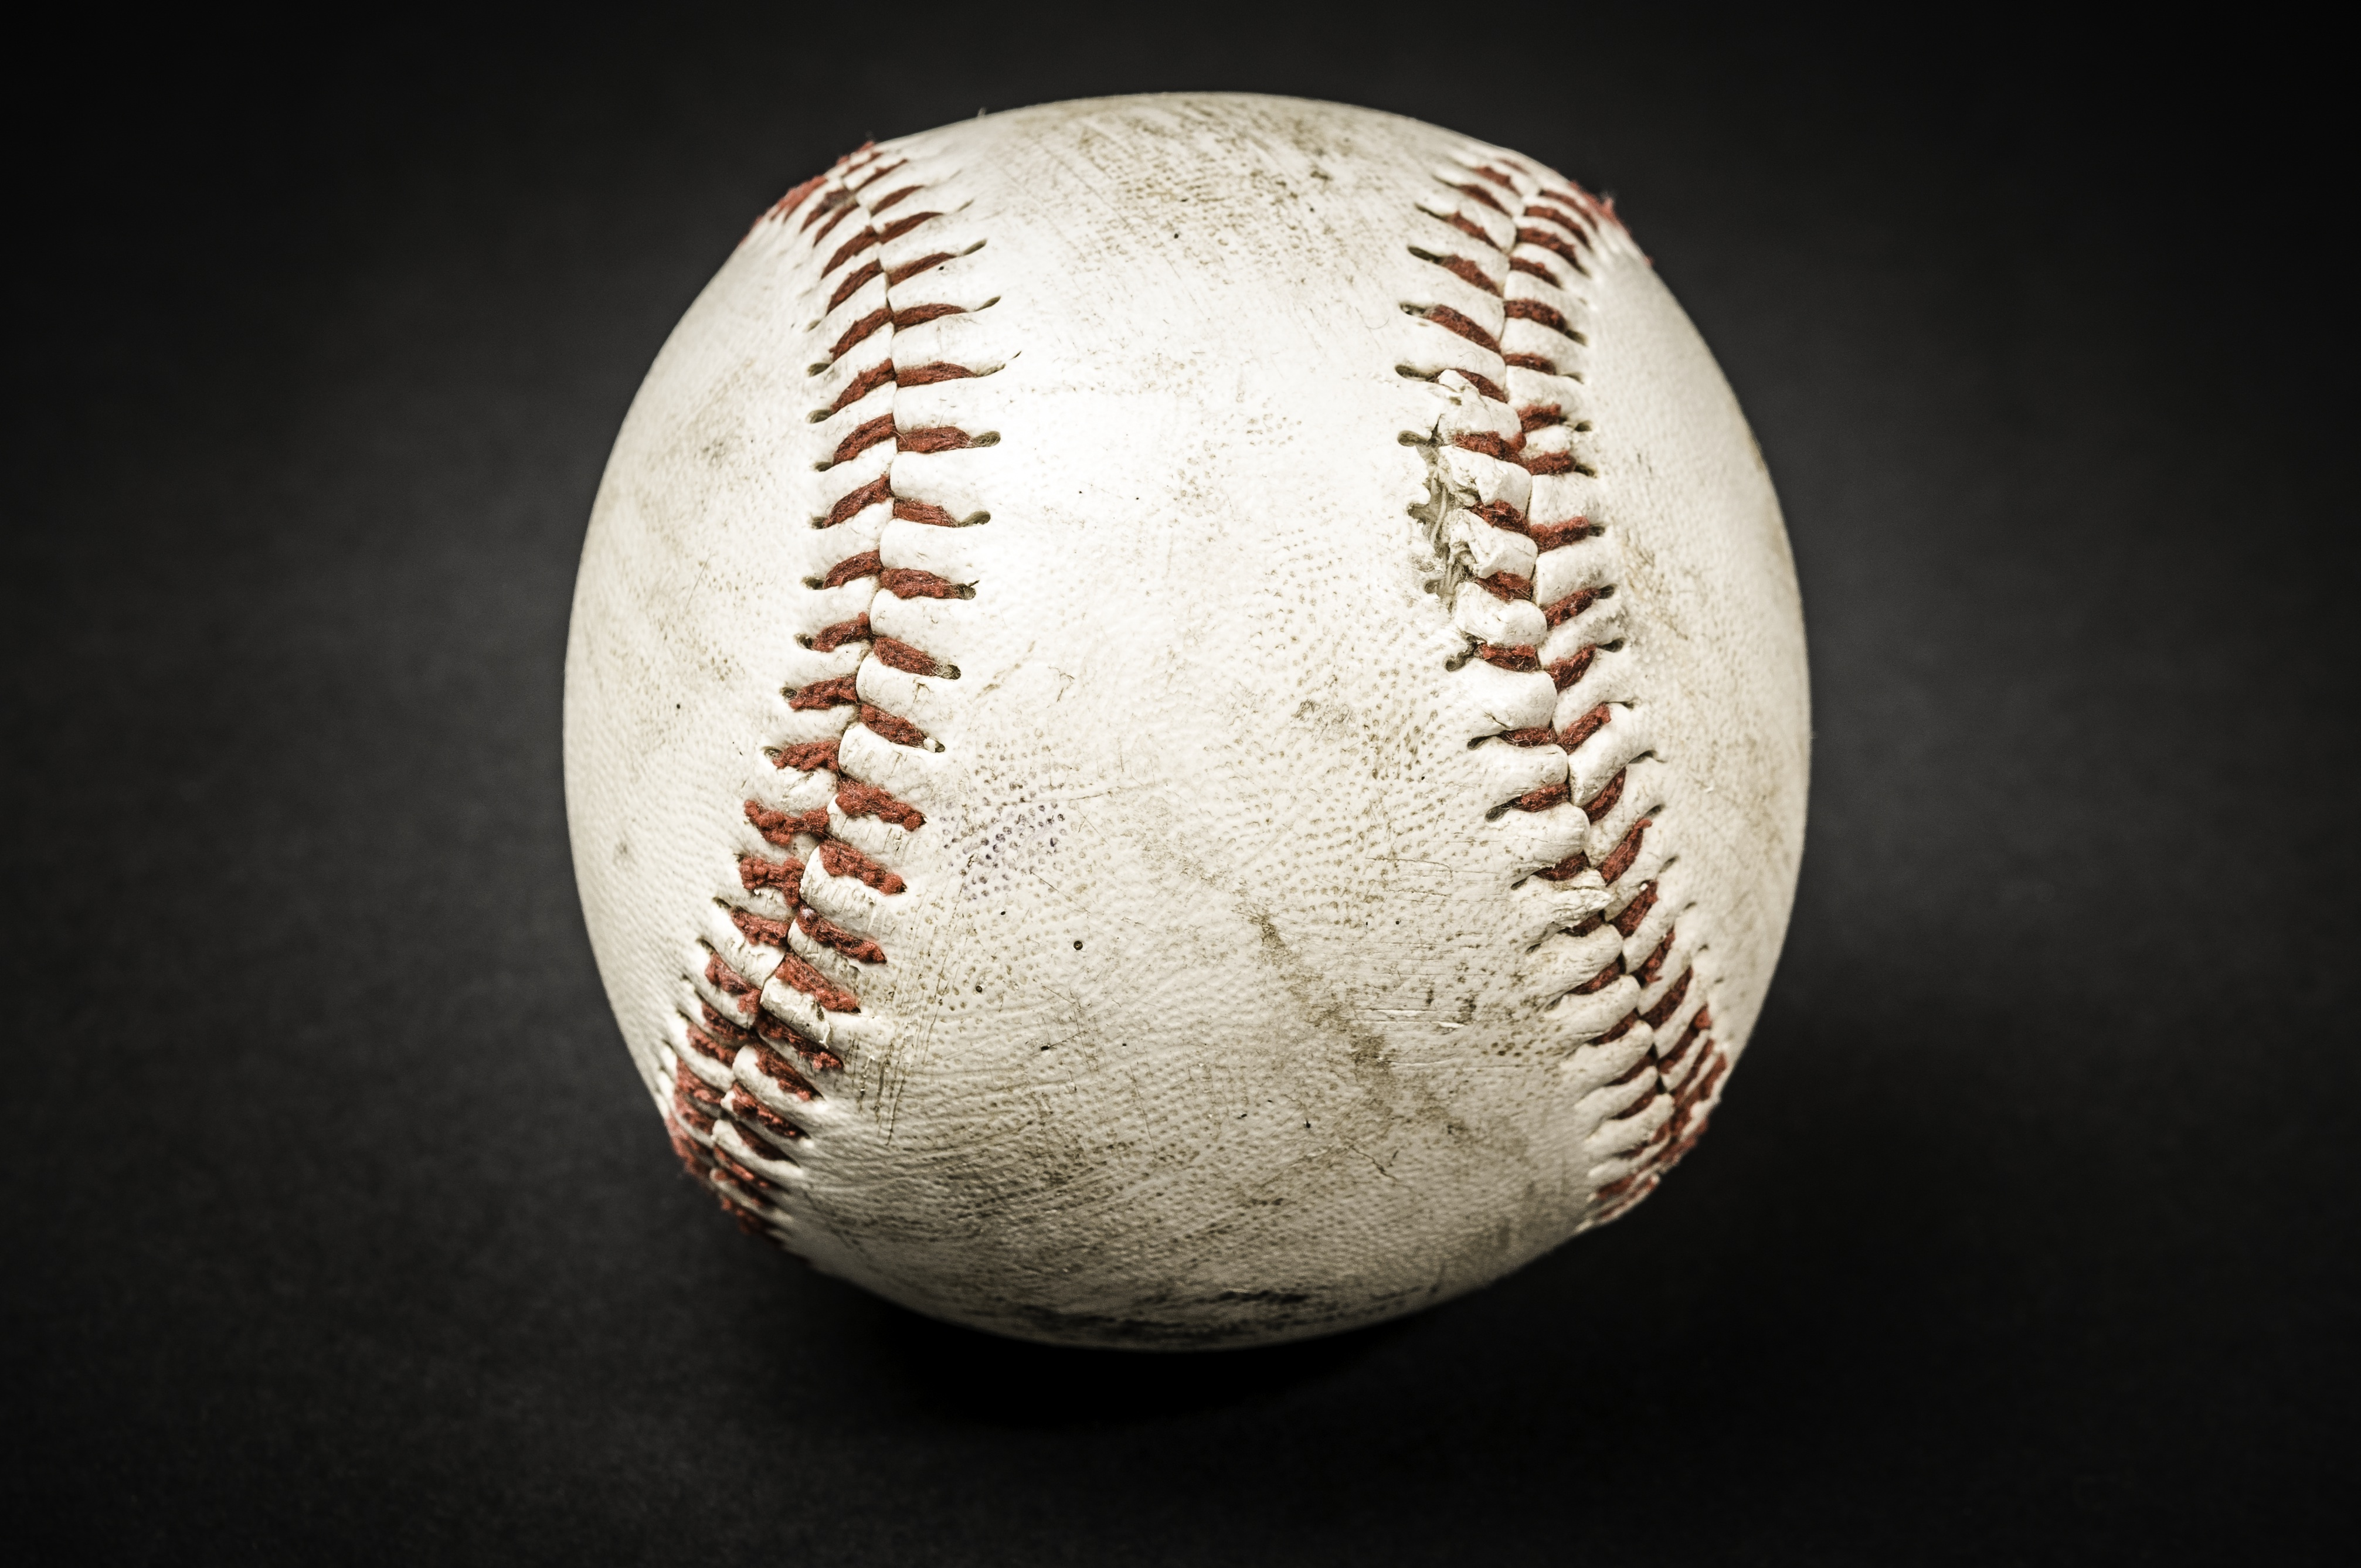
\includegraphics[width=\textwidth]{images/baseball.jpg}
  \end{center}
  \vfill%
  \fontsize{14}{16}\selectfont\par\noindent\allcaps{\thanklesspublisher}%
  \end{fullwidth}%
  }
  \thispagestyle{empty}%
  \clearpage%
}

% From "user11232" at:
% http://tex.stackexchange.com/questions/167526/how-to-write-dedication-properly

\newenvironment{dedication}
  {%\clearpage           % we want a new page          %% I commented this
   \thispagestyle{empty}% no header and footer
   \vspace*{\stretch{1}}% some space at the top
   \itshape             % the text is in italics
   \raggedleft          % flush to the right margin
  }
  {\par % end the paragraph
   \vspace{\stretch{3}} % space at bottom is three times that at the top
   \clearpage           % finish off the page
  }
